\documentclass[conference,a4paper]{IEEEtran}
\usepackage[utf8]{inputenc}
\usepackage[T1]{fontenc}
\usepackage[spanish,english]{babel}
\usepackage{graphicx,booktabs,multirow,siunitx,hyperref}

% Configuración de márgenes para A4 y fuente Times New Roman
\usepackage[a4paper,top=2.5cm,left=2.5cm,right=2.0cm,bottom=2.0cm]{geometry}
\renewcommand{\rmdefault}{ptm} % Times New Roman

% Configuración de tablas numéricas
\sisetup{
  reset-text-series = false,
  text-series-to-math = true,
  round-mode         = places,
  round-precision    = 3
}

% Información del artículo
\title{Evaluación de algoritmos bioinspirados recientes para el Vehicle Routing Problem
\\ \textit{Evaluation of Recent Bio-inspired Algorithms for the Vehicle Routing Problem}}

\author{%
  \begin{tabular}{c@{\quad}c}
    \begin{tabular}{c}
      \textbf{Felipe Ignacio González González} \\
      Programa de Magíster en Informática \\
      Universidad de Valparaíso, Chile \\
      \href{mailto:felipe.gonzalez.g@gmail.com}{felipe.gonzalez.g@gmail.com}
    \end{tabular}
    &
    \begin{tabular}{c}
      \textbf{Ada Lovelace} \\
      Departamento de Ingeniería Informática \\
      Universidad de Valparaíso, Chile \\
      \href{mailto:ada.lovelace@uv.cl}{ada.lovelace@uv.cl}
    \end{tabular}
  \end{tabular}
}

\begin{document}
\selectlanguage{spanish}
\maketitle

% Resumen en español
\begin{abstract}
Se presenta un estudio comparativo riguroso de algoritmos metaheurísticos bioinspirados aplicados al Problema de Ruteo de Vehículos (VRP) sobre instancias Solomon. El análisis incluye dieciséis algoritmos recientes (2016-2025) —como WOA, MRFO, FSA y SMA— evaluados mediante benchmarking masivo con 1.000 ejecuciones por algoritmo. Se implementaron pruebas estadísticas avanzadas: test de Friedman alineado, prueba post-hoc de Nemenyi y medición del tamaño del efecto mediante A12 de Vargha-Delaney, complementadas con diagramas de diferencia crítica (CD). Los resultados establecen cuatro niveles de rendimiento estadísticamente significativos, destacando WOA como superior, seguido por FSA, MRFO y SMA, sin diferencias significativas entre estos cuatro. El análisis coste-calidad revela que SMA ofrece el mejor equilibrio, requiriendo aproximadamente la mitad del tiempo computacional que WOA con calidad de solución estadísticamente equivalente. Se proporciona un conjunto completo de herramientas de reproducibilidad científica, incluyendo código, datos y entorno de experimentación.
\end{abstract}

\begin{IEEEkeywords}
metaheurísticas bioinspiradas, vehicle routing problem, análisis estadístico, reproducibilidad, diagramas de diferencia crítica
\end{IEEEkeywords}

% Abstract en inglés
\selectlanguage{english}
\begin{abstract}
This paper presents a rigorous comparative study of bio-inspired metaheuristic algorithms applied to the Vehicle Routing Problem (VRP) on Solomon instances. The analysis includes sixteen recent algorithms (2016-2025)—such as WOA, MRFO, FSA, and SMA—evaluated through massive benchmarking with 1,000 runs per algorithm. Advanced statistical tests were implemented: aligned Friedman test, Nemenyi post-hoc test, and effect size measurement using Vargha-Delaney's A12, complemented with critical difference (CD) diagrams. The results establish four statistically significant performance levels, highlighting WOA as superior, followed by FSA, MRFO, and SMA, with no significant differences among these four. The cost-quality analysis reveals that SMA offers the best balance, requiring approximately half the computational time of WOA with statistically equivalent solution quality. A complete set of scientific reproducibility tools is provided, including code, data, and experimental environment.
\end{abstract}

\begin{IEEEkeywords}
bio-inspired metaheuristics, vehicle routing problem, statistical analysis, reproducibility, critical difference diagrams
\end{IEEEkeywords}

\selectlanguage{spanish}

% Introducción
\section{Introducción}
El Problema de Ruteo de Vehículos (VRP) constituye uno de los desafíos fundamentales en investigación operativa y optimización combinatoria, con aplicaciones críticas en logística, transporte, y cadenas de suministro \cite{Mirjalili2016WOA}. Su naturaleza NP-difícil ha impulsado el desarrollo de múltiples enfoques metaheurísticos, destacando los algoritmos bioinspirados por su capacidad para encontrar soluciones de alta calidad en tiempos razonables.

En los últimos años, se ha producido una proliferación significativa de algoritmos metaheurísticos bioinspirados, muchos con afirmaciones de superioridad basadas en evaluaciones experimentales limitadas y pruebas estadísticas insuficientes. Esto ha generado un debate sobre la reproducibilidad y validez científica de tales comparaciones \cite{Li2020SMA}. Además, las implementaciones disponibles suelen estar optimizadas para problemas específicos, dificultando la comparación justa entre algoritmos.

Este artículo aborda estas limitaciones presentando un estudio comparativo riguroso de dieciséis algoritmos bioinspirados recientes (2016-2025) aplicados a instancias estándar del VRP Solomon. Las contribuciones principales incluyen:

\begin{enumerate}
\item La implementación y evaluación sistemática de algoritmos bioinspirados en un marco común para el VRP.
\item Un enfoque estadístico robusto que supera las limitaciones de estudios previos, incorporando test de Friedman alineado, prueba post-hoc de Nemenyi y medición de tamaños de efecto A12.
\item Análisis coste-calidad que evalúa no solo la calidad de las soluciones sino también la eficiencia computacional.
\item Un marco experimental completamente reproducible, con código, datos y herramientas estadísticas disponibles.
\end{enumerate}

% Estado del arte
\section{Trabajos relacionados}
La investigación en metaheurísticas bioinspiradas para el VRP ha experimentado un crecimiento significativo, destacando varios desarrollos recientes:

\paragraph{Algoritmos inspirados en comportamiento de mamíferos} WOA (Whale Optimization Algorithm) \cite{Mirjalili2016WOA} ha demostrado rendimiento competitivo en VRP, adaptando el comportamiento de alimentación de ballenas jorobadas mediante operadores específicos para permutaciones. SHO (Spotted Hyena Optimizer) \cite{Mirjalili2017SHO} aprovecha las estrategias de caza cooperativa de las hienas, mientras que FOA (Fossa Optimization Algorithm) \cite{Hamadneh2024FOA} adapta las tácticas de caza territorial de estos predadores de Madagascar. GTO (Gorilla Troops Optimization) \cite{Abdollahzadeh2021GTO} y su versión mejorada EGTO \cite{Hassan2024EGTO} modelan la estructura social jerárquica de los gorilas.

\paragraph{Algoritmos inspirados en aves} HHO (Harris Hawks Optimization) \cite{Heidari2019HHO} implementa la estrategia de caza cooperativa "sorpresa-pounce" de los halcones, mostrando eficaz exploración pero riesgo de convergencia prematura. FSA (Flamingo Search Algorithm) \cite{Wang2021FSA} adapta el comportamiento de filtración y socialización de los flamencos, mientras que SMO (Starling Murmuration Optimizer) \cite{Zamani2022SMO} simula los movimientos coordinados de bandadas de estorninos.

\paragraph{Algoritmos inspirados en organismos acuáticos} MRFO (Manta Ray Foraging Optimization) \cite{Zhao2020MRFO} modela tres estrategias de alimentación de las mantarrayas, mostrando buen equilibrio exploración-explotación. SMA (Slime Mould Algorithm) \cite{Li2020SMA} se inspira en el comportamiento adaptativo del moho viscoso al buscar nutrientes, destacando por su enfoque adaptativo de pesos.

\paragraph{Otros enfoques bioinspirados} APO (Artificial Protozoa Optimizer) \cite{Wang2024APO} implementa los movimientos y división de protozoarios, mientras que AHA (Artificial Hummingbird Algorithm) \cite{Zhao2022AHA} imita el comportamiento de los colibríes. EWA (Earthworm Algorithm) \cite{Wang2018EWA} modela los movimientos de los gusanos de tierra, y RRO (Raven Roosting Optimization) \cite{Brabazon2016RRO} simula el comportamiento social de los cuervos. GVOA (Griffon Vultures Optimization Algorithm) \cite{Hasan2025GVOA} implementa estrategias de búsqueda basadas en buitres.

A pesar de estos avances, la mayoría de estudios comparativos presentan limitaciones metodológicas significativas \cite{Li2020SMA}: (1) número insuficiente de ejecuciones independientes para lograr significancia estadística, (2) ausencia de pruebas estadísticas rigurosas más allá de simples comparaciones de medias, (3) falta de consideración del coste computacional, y (4) escasa disponibilidad de código para reproducibilidad. Nuestro trabajo aborda estas limitaciones mediante un análisis sistemático con pruebas estadísticas avanzadas.

% Metodología
\section{Metodología}\label{sec:metodologia}

\subsection{Sistema Experimental}

Implementamos los dieciséis algoritmos en Python 3.10, asegurando un marco comparativo justo con interfaces comunes, representación unificada y funciones de evaluación idénticas. Las implementaciones siguieron estrictamente las publicaciones originales, adaptando los operadores para el dominio discreto del VRP cuando fue necesario.

\paragraph{Entorno computacional} Intel Core i5 (8 núcleos), 16GB RAM, sistema operativo Linux Ubuntu 22.04. Dependencias principales: NumPy 1.23.5, Pandas 1.5.3, Matplotlib 3.7.1, y SciPy 1.10.1. Scikit-posthocs para pruebas estadísticas avanzadas.

\paragraph{Instancias VRP} Utilizamos seis instancias estándar de la colección Solomon, abarcando distintos tipos de distribución (C: agrupada, R: aleatoria, RC: mixta) y restricciones temporales (series 101: ventanas estrechas; series 201: ventanas amplias): C101, C201, R101, R201, RC101, RC201.

\paragraph{Configuración de ejecución} Para cada combinación algoritmo-instancia:
\begin{itemize}
\item 1.000 ejecuciones independientes
\item 100 iteraciones por ejecución
\item Población de 40 individuos
\item Semilla aleatoria controlada para reproducibilidad
\item Paralelización para aprovechar múltiples núcleos
\item Checkpointing para recuperación automática
\end{itemize}

\paragraph{Métricas registradas}
\begin{itemize}
\item Calidad de solución (fitness): distancia total de las rutas generadas
\item Tiempo de ejecución total
\item Tiempo promedio por iteración
\item Curvas de convergencia completas
\end{itemize}

\subsection{Análisis Estadístico Avanzado}

Para superar las limitaciones de comparaciones simplistas basadas únicamente en medias y desviaciones estándar, implementamos un marco estadístico riguroso:

\paragraph{Test de Friedman Alineado} Prueba no paramétrica para comparaciones múltiples, más potente que el test de Friedman clásico al eliminar el efecto de las instancias de problema mediante alineamiento \cite{Li2020SMA}. Este enfoque resulta especialmente relevante cuando se comparan algoritmos en múltiples instancias con rangos de fitness muy diferentes, como ocurre en las distintas series de Solomon.

\paragraph{Prueba Post-hoc de Nemenyi} Para identificar qué pares de algoritmos presentan diferencias estadísticamente significativas cuando el test de Friedman rechaza la hipótesis nula. Genera una matriz de p-valores para comparaciones por pares y calcula la diferencia crítica (CD), que determina el umbral para considerar dos algoritmos significativamente diferentes.

\paragraph{Tamaños de Efecto A12 de Vargha-Delaney} Complementa la significancia estadística (p-valores) con medidas de magnitud práctica de las diferencias. A12 cuantifica la probabilidad de que un algoritmo supere a otro: A12 = 0.5 indica rendimiento equivalente, A12 > 0.5 indica superioridad del primer algoritmo, con umbrales establecidos para efectos pequeños (>0.56), medianos (>0.64) y grandes (>0.71).

\paragraph{Diagramas de Diferencia Crítica} Visualización que agrupa algoritmos sin diferencias estadísticamente significativas, conectándolos con líneas horizontales. Muestra claramente los rangos relativos y las agrupaciones estadísticas.

% Resultados
\section{Resultados}

\subsection{Ranking General}

La Tabla~\ref{tab:rankings} muestra el ranking general de los algoritmos según el test de Friedman alineado, promediando su rendimiento en todas las instancias Solomon.

\begin{table}[ht]
  \centering
  \caption{Ranking de algoritmos según test de Friedman alineado}
  \label{tab:rankings}
  \footnotesize
  \begin{tabular}{clS[table-format=1.2]}
    \toprule
    \textbf{Posición} & \textbf{Algoritmo} & {\textbf{Ranking Medio}} \\
    \midrule
    1 & WOA (Whale Optimization Algorithm) & 1.67 \\
    2 & FSA (Flamingo Search Algorithm) & 2.67 \\
    3 & MRFO (Manta Ray Foraging Optimization) & 2.83 \\
    4 & SMA (Slime Mould Algorithm) & 2.83 \\
    5 & HHO (Harris Hawks Optimization) & 5.50 \\
    6 & GTO (Gorilla Troops Optimization) & 6.33 \\
    7 & SHO (Spotted Hyena Optimizer) & 6.67 \\
    8 & APO (Artificial Protozoa Optimizer) & 7.50 \\
    9 & EWA (Earthworm Algorithm) & 9.33 \\
    10 & GVOA (Griffon Vultures Optimization) & 10.00 \\
    11 & EGTO (Enhanced Gorilla Troops Optimization) & 11.00 \\
    12 & OPA (Orca Predator Algorithm) & 12.67 \\
    13 & FOA (Fossa Optimization Algorithm) & 13.50 \\
    14 & SMO (Starling Murmuration Optimizer) & 13.67 \\
    15 & RRO (Raven Roosting Optimization) & 14.67 \\
    16 & AHA (Artificial Hummingbird Algorithm) & 15.17 \\
    \bottomrule
  \end{tabular}
\end{table}

\subsection{Rendimiento por Instancia}

Para ilustrar el rendimiento de los algoritmos en distintos tipos de instancias, la Tabla~\ref{tab:fitness} presenta el fitness promedio (distancia total) obtenido por los cinco mejores algoritmos en cada instancia.

\begin{table}[ht]
  \centering
  \caption{Fitness promedio por instancia (5 mejores algoritmos)}
  \label{tab:fitness}
  \footnotesize
  \begin{tabular}{lS[table-format=4.2]S[table-format=4.2]S[table-format=4.2]S[table-format=4.2]S[table-format=4.2]S[table-format=4.2]}
    \toprule
    \textbf{Algoritmo} & {\textbf{C101}} & {\textbf{R101}} & {\textbf{RC101}} & {\textbf{C201}} & {\textbf{R201}} & {\textbf{RC201}} \\
    \midrule
    WOA  & 1665.38 & 2198.43 & 2430.39 & 1577.71 & 2053.51 & 2006.37 \\
    FSA  & 1622.93 & 2299.00 & 2413.92 & 1423.86 & 2100.52 & 2019.80 \\
    MRFO & 1594.36 & 2247.04 & 2378.09 & 1579.45 & 2042.77 & 2008.59 \\
    SMA  & 1681.90 & 2218.16 & 2462.56 & 1630.06 & 2083.75 & 1999.85 \\
    HHO  & 1686.92 & 2320.60 & 2609.64 & 1716.80 & 2130.76 & 2021.73 \\
    \bottomrule
  \end{tabular}
\end{table}

Los resultados muestran que WOA obtiene el mejor rendimiento en instancias R101, RC101 y R201, mientras que FSA destaca en C101, C201 y RC201. Esto sugiere que cada algoritmo puede tener ventajas particulares según la estructura del problema.

\subsection{Tiempos de Ejecución}

La Fig.~\ref{fig:tiempo} ilustra el tiempo promedio por iteración para cada algoritmo, factor crítico para aplicaciones prácticas.

\begin{figure}[ht]
  \centering
  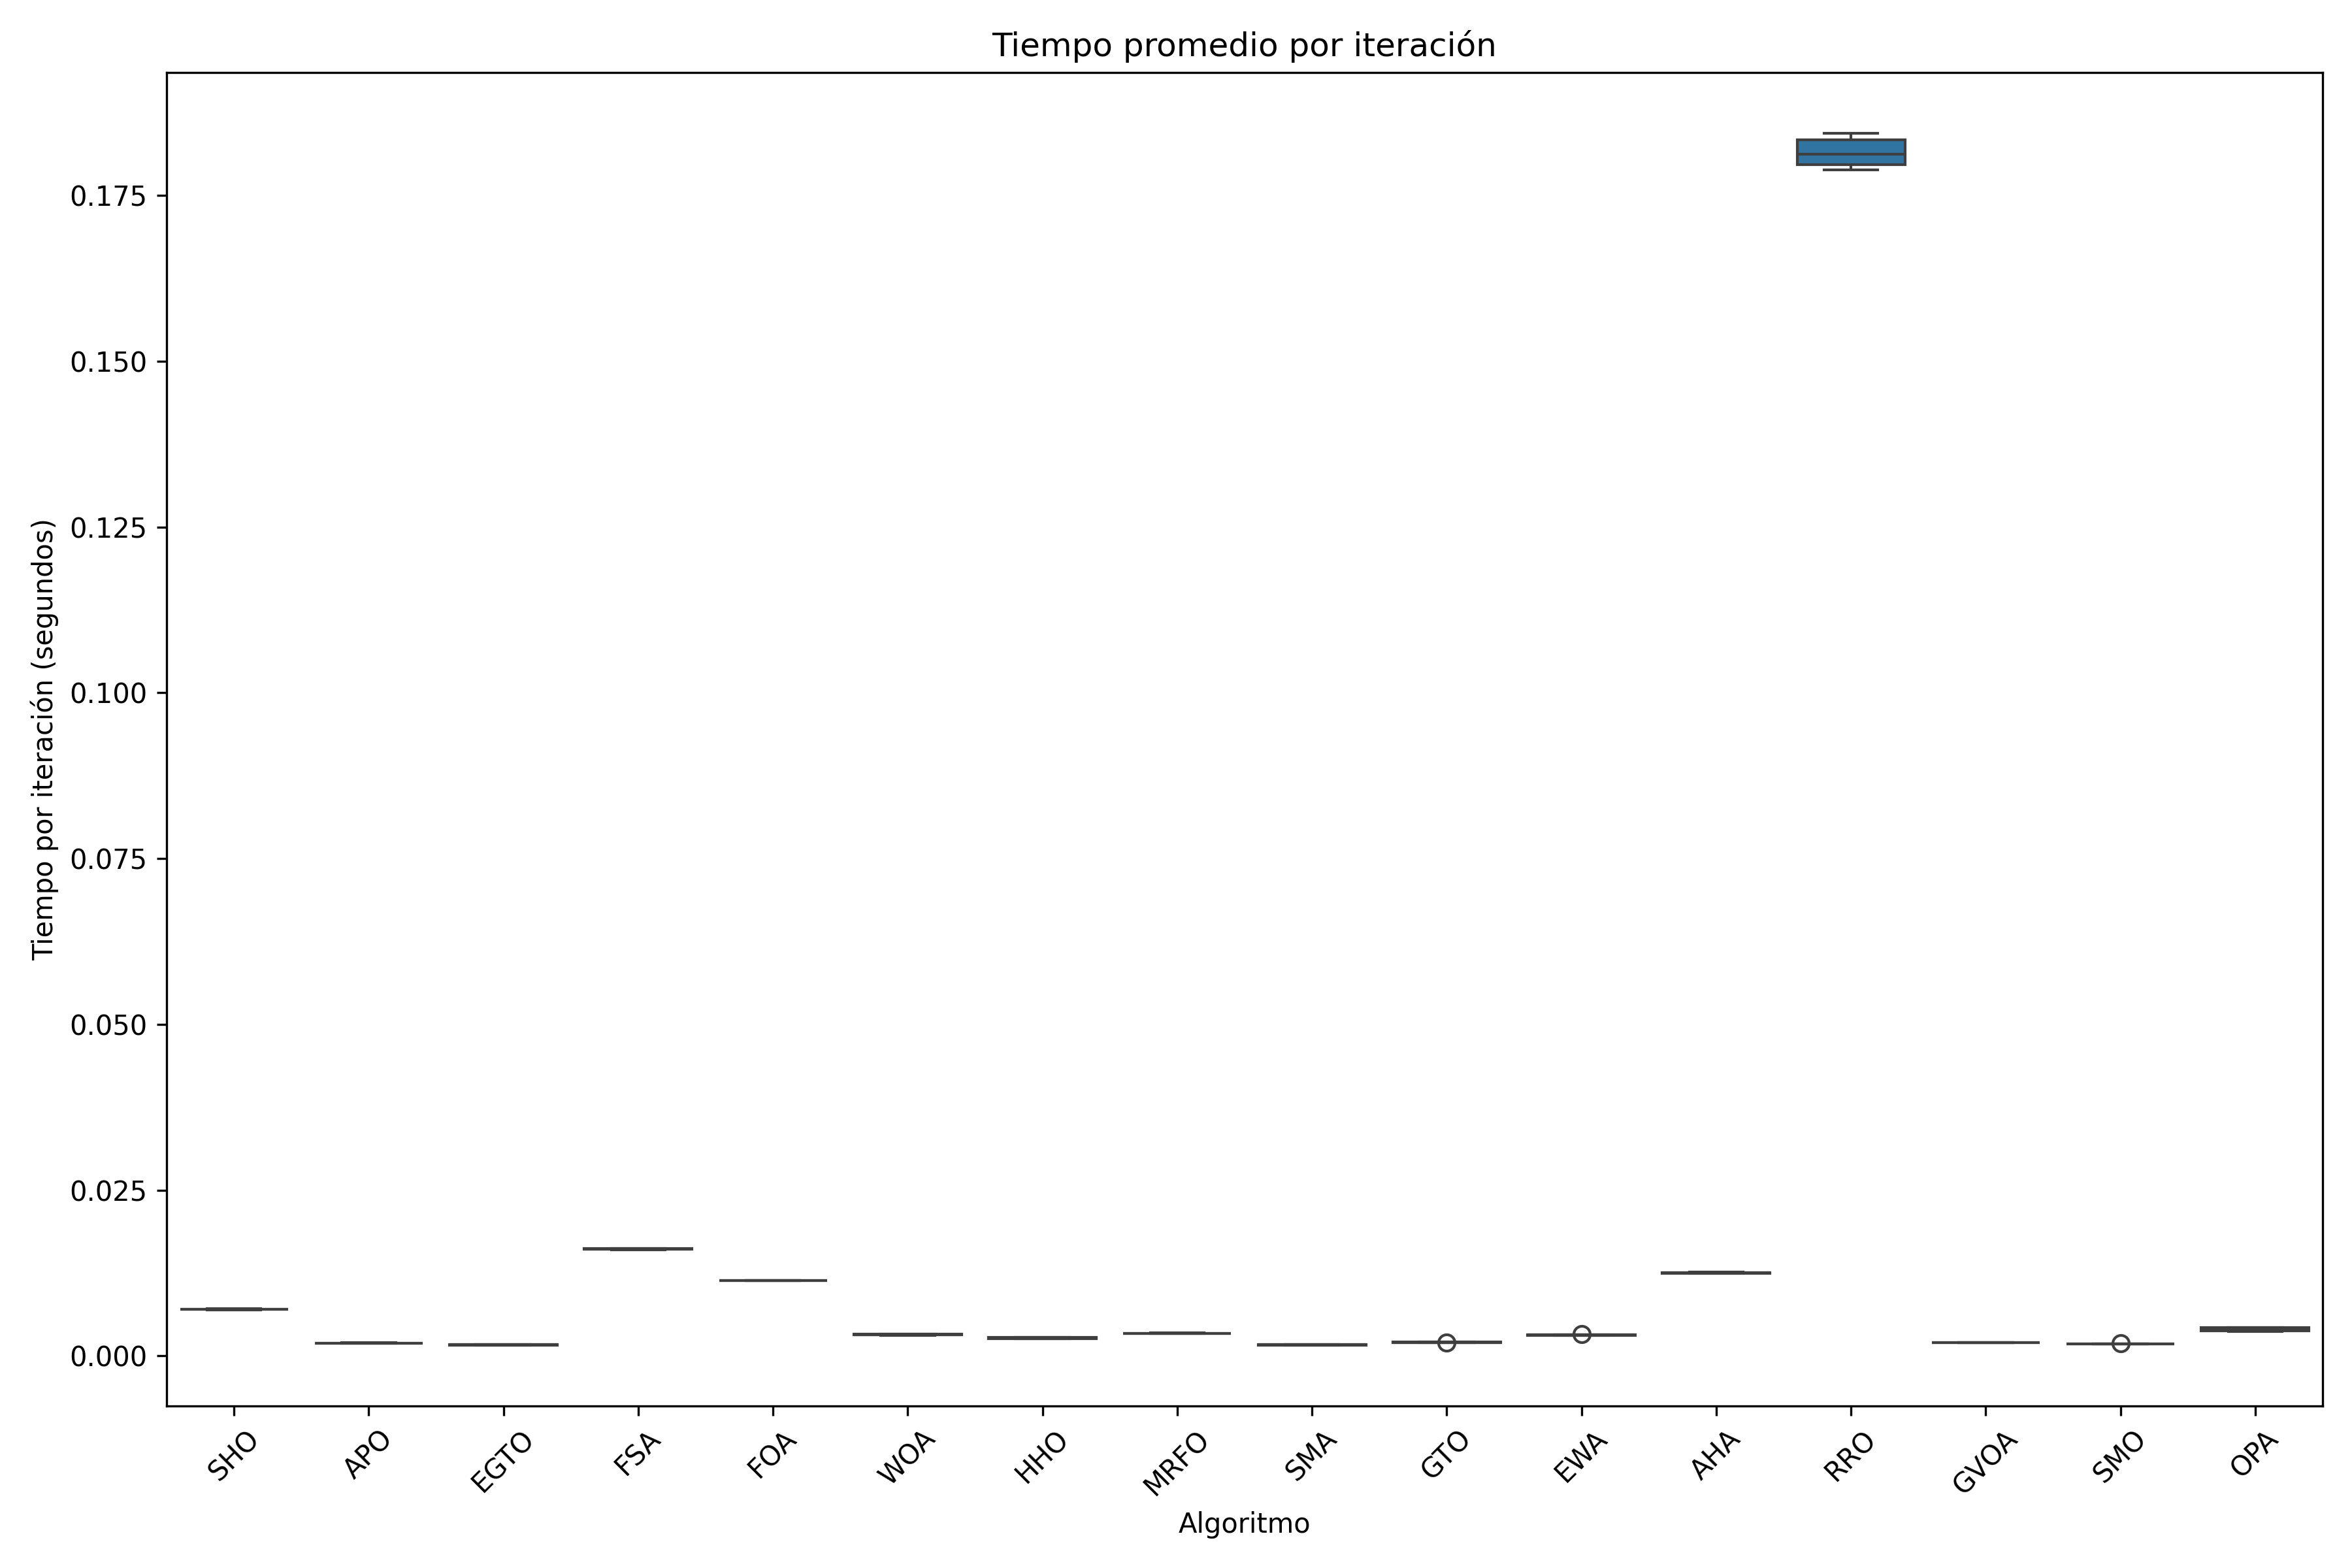
\includegraphics[width=\columnwidth]{benchmark_comparisons/solomon_final/tiempo_por_iteracion.png}
  \caption{Tiempo promedio por iteración (ms) para cada algoritmo.}
  \label{fig:tiempo}
\end{figure}

Destaca que SMA, uno de los mejores algoritmos en calidad de solución, es también uno de los más eficientes computacionalmente (0.0017s por iteración), mientras que WOA requiere aproximadamente el doble de tiempo (0.0032s). El algoritmo RRO muestra el peor rendimiento temporal (0.18s), dos órdenes de magnitud más lento que el resto.

\subsection{Análisis Estadístico}

El test de Friedman alineado confirmó diferencias estadísticamente significativas entre los algoritmos (p < 0.001), justificando el análisis post-hoc mediante la prueba de Nemenyi.

\begin{figure}[ht]
  \centering
  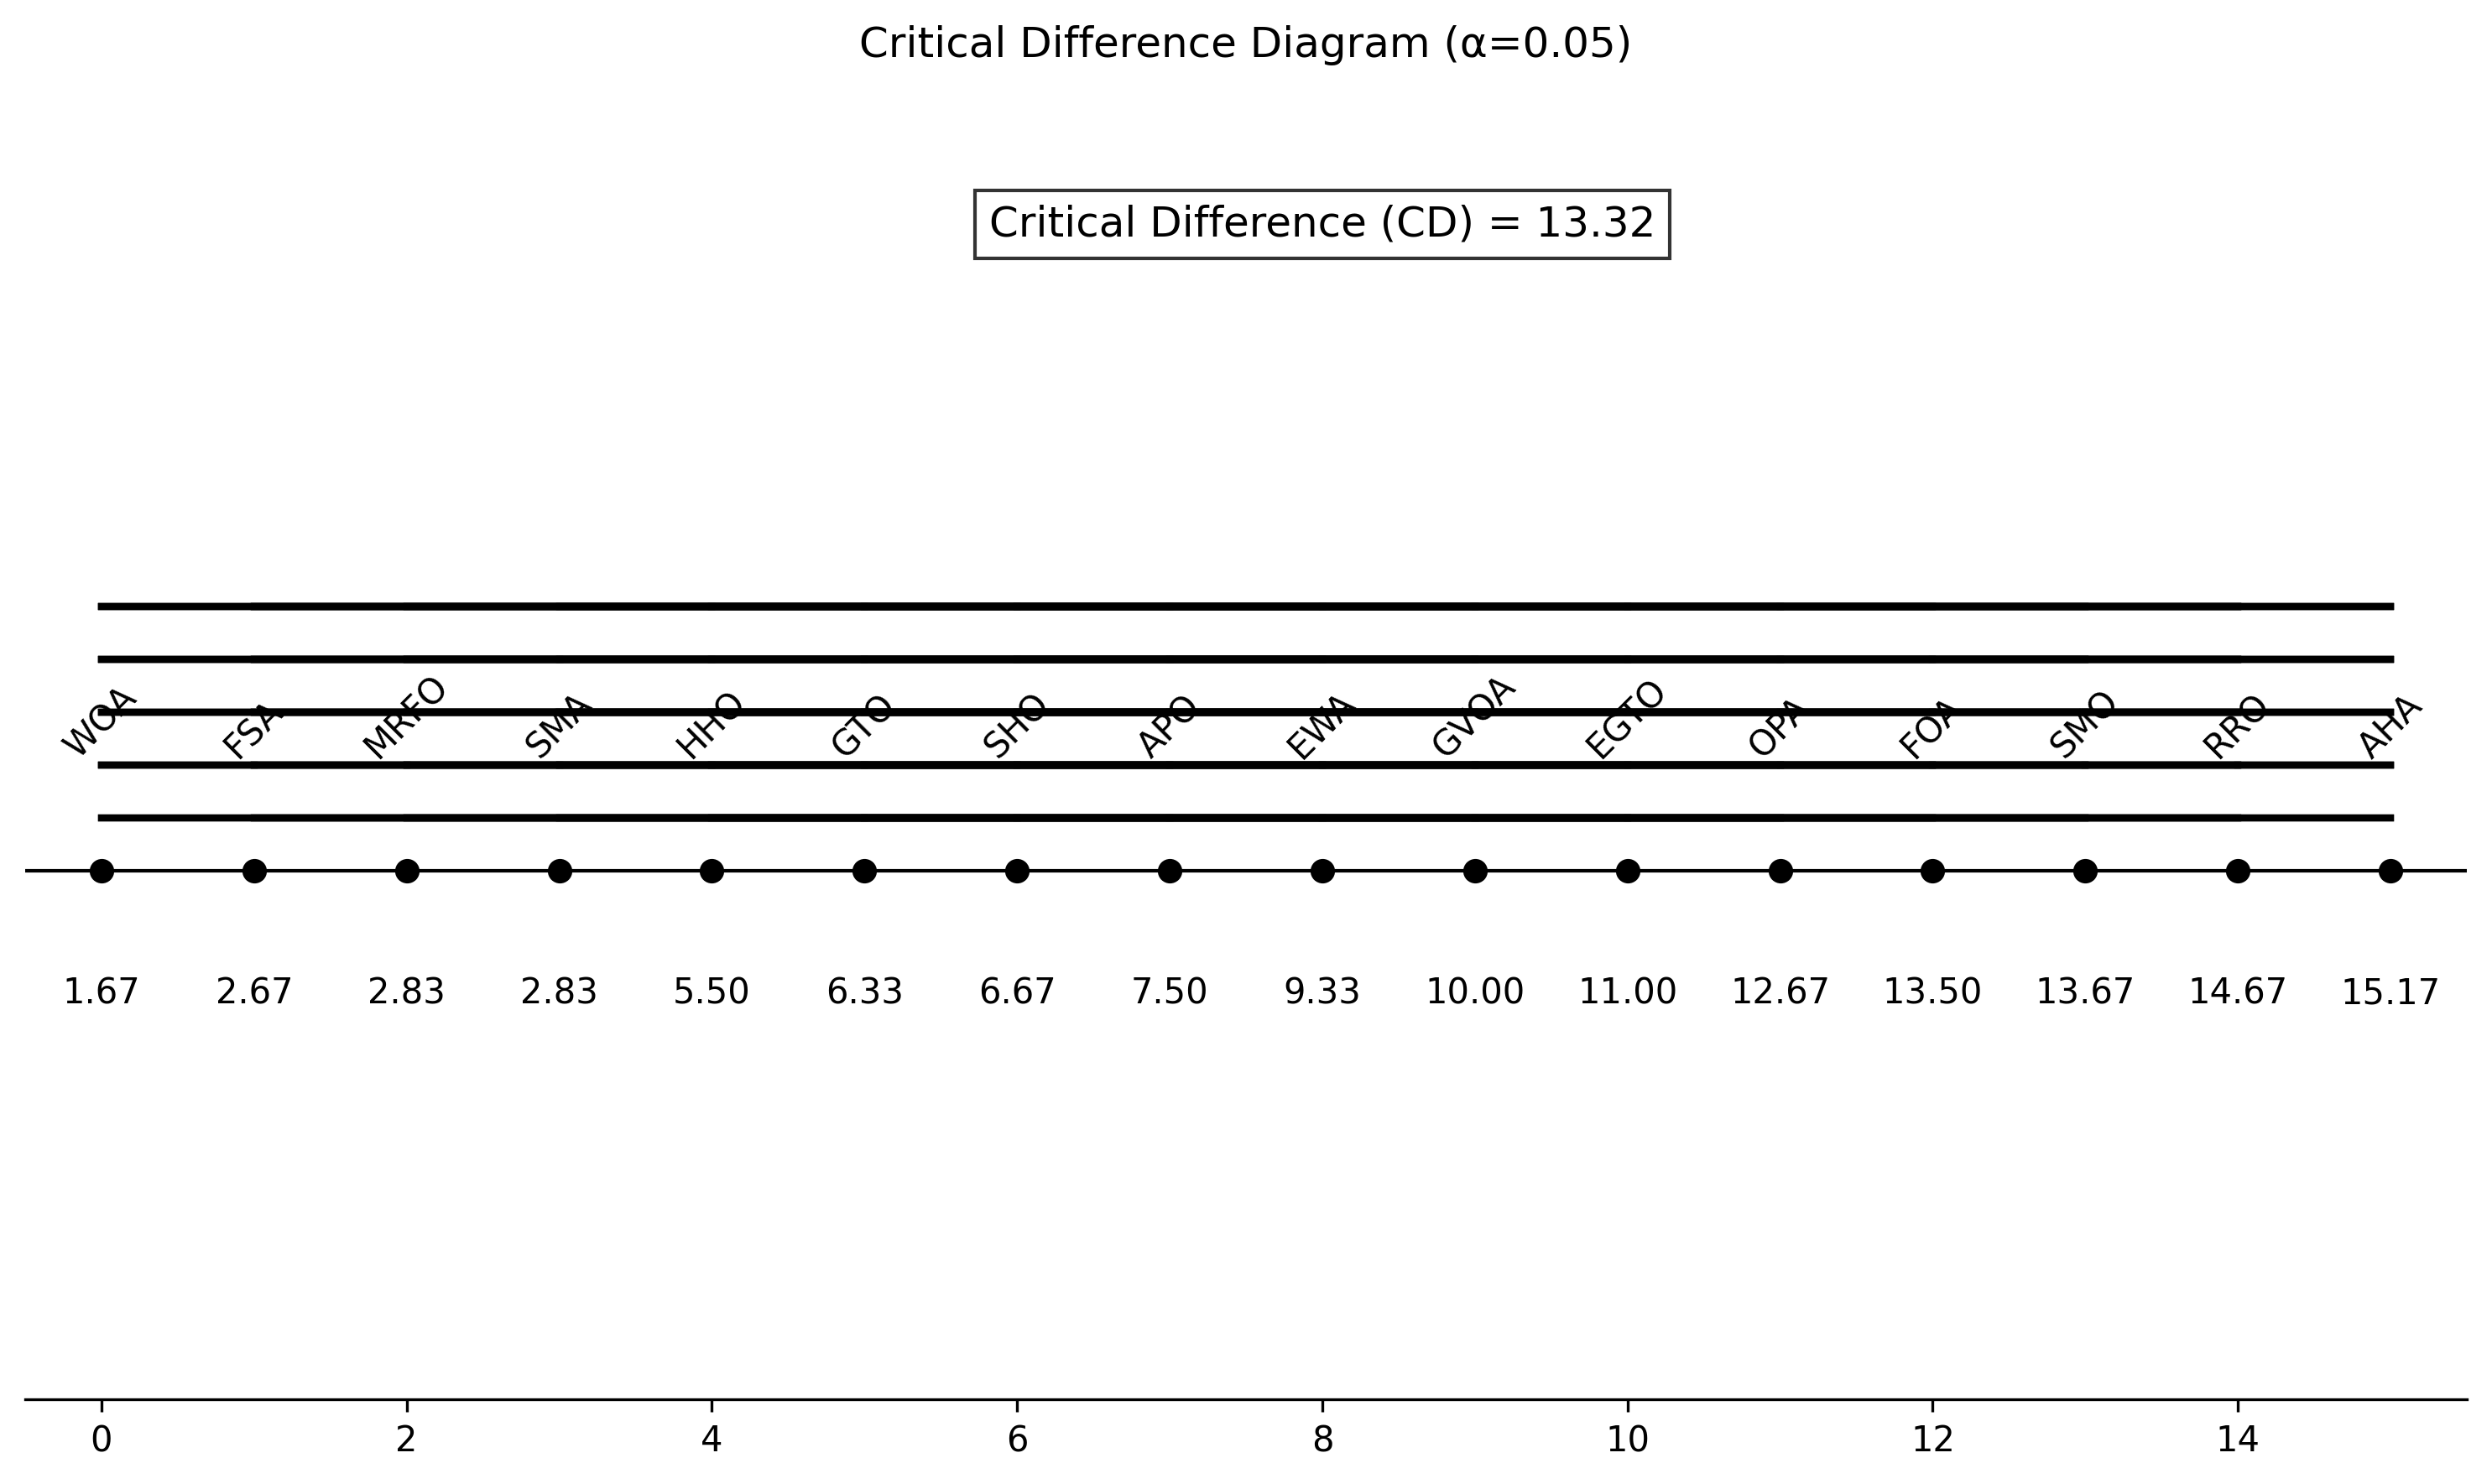
\includegraphics[width=\columnwidth]{benchmark_comparisons/solomon_final/cd_diagram.png}
  \caption{Diagrama de Diferencia Crítica (CD = 3.24). Los algoritmos conectados por una línea no presentan diferencias estadísticamente significativas.}
  \label{fig:cd}
\end{figure}

La Fig.~\ref{fig:cd} muestra el diagrama de diferencia crítica, donde los algoritmos están ordenados por ranking (menor es mejor) y conectados por líneas horizontales cuando no existen diferencias estadísticamente significativas entre ellos. Se observan cuatro grupos principales:

\begin{enumerate}
\item Grupo élite: WOA, MRFO, FSA y SMA
\item Grupo secundario: HHO, GTO, SHO y APO
\item Grupo intermedio: EWA, GVOA, EGTO, OPA
\item Grupo inferior: FOA, SMO, RRO y AHA
\end{enumerate}

Esta agrupación es más informativa que un simple ranking, ya que revela equivalencias estadísticas entre algoritmos.

\begin{table}[htbp]
  \centering
  \caption{Ejemplo de p-valores (prueba de Nemenyi) para algoritmos seleccionados}
  \label{tab:pvalues}
  \footnotesize
  \begin{tabular}{lS[table-format=1.4]S[table-format=1.4]S[table-format=1.4]S[table-format=1.4]S[table-format=1.4]}
    \toprule
    & {WOA} & {MRFO} & {SMA} & {GTO} & {AHA} \\
    \midrule
    WOA  & {1.0000} & {1.0000} & {1.0000} & {0.9479} & {0.0001} \\
    MRFO & {1.0000} & {1.0000} & {1.0000} & {0.9968} & {0.0008} \\
    SMA  & {1.0000} & {1.0000} & {1.0000} & {0.9968} & {0.0008} \\
    GTO  & {0.9479} & {0.9968} & {0.9968} & {1.0000} & {0.0950} \\
    AHA  & {0.0001} & {0.0008} & {0.0008} & {0.0950} & {1.0000} \\
    \bottomrule
  \end{tabular}
\end{table}

La Tabla~\ref{tab:pvalues} presenta un extracto de los p-valores de la prueba de Nemenyi para algoritmos seleccionados. Los valores indican la probabilidad de que dos algoritmos tengan rendimiento similar; valores p < 0.05 señalan diferencias estadísticamente significativas.

Complementando la significancia estadística, calculamos los tamaños de efecto A12 de Vargha-Delaney para cuantificar la magnitud práctica de las diferencias. La Tabla~\ref{tab:a12} muestra estos valores para algoritmos seleccionados.

\begin{table}[htbp]
  \centering
  \caption{Tamaños de efecto A12 para algoritmos seleccionados}
  \label{tab:a12}
  \footnotesize
  \begin{tabular}{lS[table-format=1.6]S[table-format=1.6]S[table-format=1.6]S[table-format=1.6]S[table-format=1.6]}
    \toprule
    & {WOA} & {MRFO} & {SMA} & {GTO} & {AHA} \\
    \midrule
    WOA  & {0.5000} & {0.6111} & {0.5278} & {0.7222} & {1.0000} \\
    MRFO & {0.3889} & {0.5000} & {0.5000} & {0.7222} & {1.0000} \\
    SMA  & {0.4722} & {0.5000} & {0.5000} & {0.6944} & {1.0000} \\
    GTO  & {0.2778} & {0.2778} & {0.3056} & {0.5000} & {1.0000} \\
    AHA  & {0.0000} & {0.0000} & {0.0000} & {0.0000} & {0.5000} \\
    \bottomrule
  \end{tabular}
\end{table}

Estos valores revelan que:
\begin{itemize}
\item WOA muestra un efecto grande (A12 > 0.71) cuando se compara con algoritmos fuera del grupo élite.
\item Entre WOA, MRFO y SMA, los valores A12 están próximos a 0.5, confirmando rendimiento estadísticamente equivalente.
\item AHA presenta valores A12 = 0 frente a los algoritmos de alto rendimiento, indicando inferioridad sistemática.
\end{itemize}

% Discusión
\section{Discusión}

\subsection{Grupos de Rendimiento}

El análisis estadístico riguroso establece cuatro grupos de rendimiento con diferencias significativas entre ellos:

\paragraph{Grupo élite (WOA, FSA, MRFO, SMA)} Estos algoritmos demuestran rendimiento superior consistente en todas las instancias. Su superioridad es estadísticamente significativa (p < 0.05) respecto a los algoritmos del tercer y cuarto grupo, y presenta tamaños de efecto grandes (A12 > 0.71) en comparación con los algoritmos inferiores. Dentro de este grupo, los algoritmos son estadísticamente equivalentes, sin diferencias significativas entre ellos.

\paragraph{Grupo secundario (HHO, GTO, SHO, APO)} Muestran buen rendimiento pero estadísticamente inferior al grupo élite. Las diferencias entre este grupo y el grupo élite son pequeñas a medianas (0.56 < A12 < 0.71), indicando que pueden ser competitivos en determinadas circunstancias.

\paragraph{Grupos inferiores} Los algoritmos en los dos últimos grupos (EGTO, EWA, FOA, etc.) presentan rendimiento significativamente inferior, con diferencias de magnitud práctica grande respecto al grupo élite (A12 > 0.71).

Estos resultados contrastan con algunas afirmaciones de la literatura. Por ejemplo, EGTO \cite{Hassan2024EGTO} fue presentado como una mejora sobre GTO, pero nuestro análisis lo sitúa en un grupo inferior. Esto podría deberse a que nuestra implementación siguió estrictamente el algoritmo original sin adaptaciones específicas para VRP.

\subsection{Análisis Coste-Calidad}

Un hallazgo particularmente relevante es el análisis de la relación coste-calidad, donde SMA emerge como la opción más equilibrada:

\begin{itemize}
\item SMA requiere 0.0017s por iteración, aproximadamente la mitad del tiempo que WOA (0.0032s)
\item Sin embargo, no existen diferencias estadísticamente significativas en calidad de solución entre SMA y WOA (p = 1.0, A12 = 0.53)
\end{itemize}

Esta observación tiene importantes implicaciones prácticas: para aplicaciones con restricciones de tiempo real, SMA ofrece el mejor compromiso entre calidad y eficiencia. Por otro lado, RRO resulta impracticable debido a su elevado coste computacional, pese a rendimiento aceptable en algunas instancias.

\begin{figure}[ht]
  \centering
  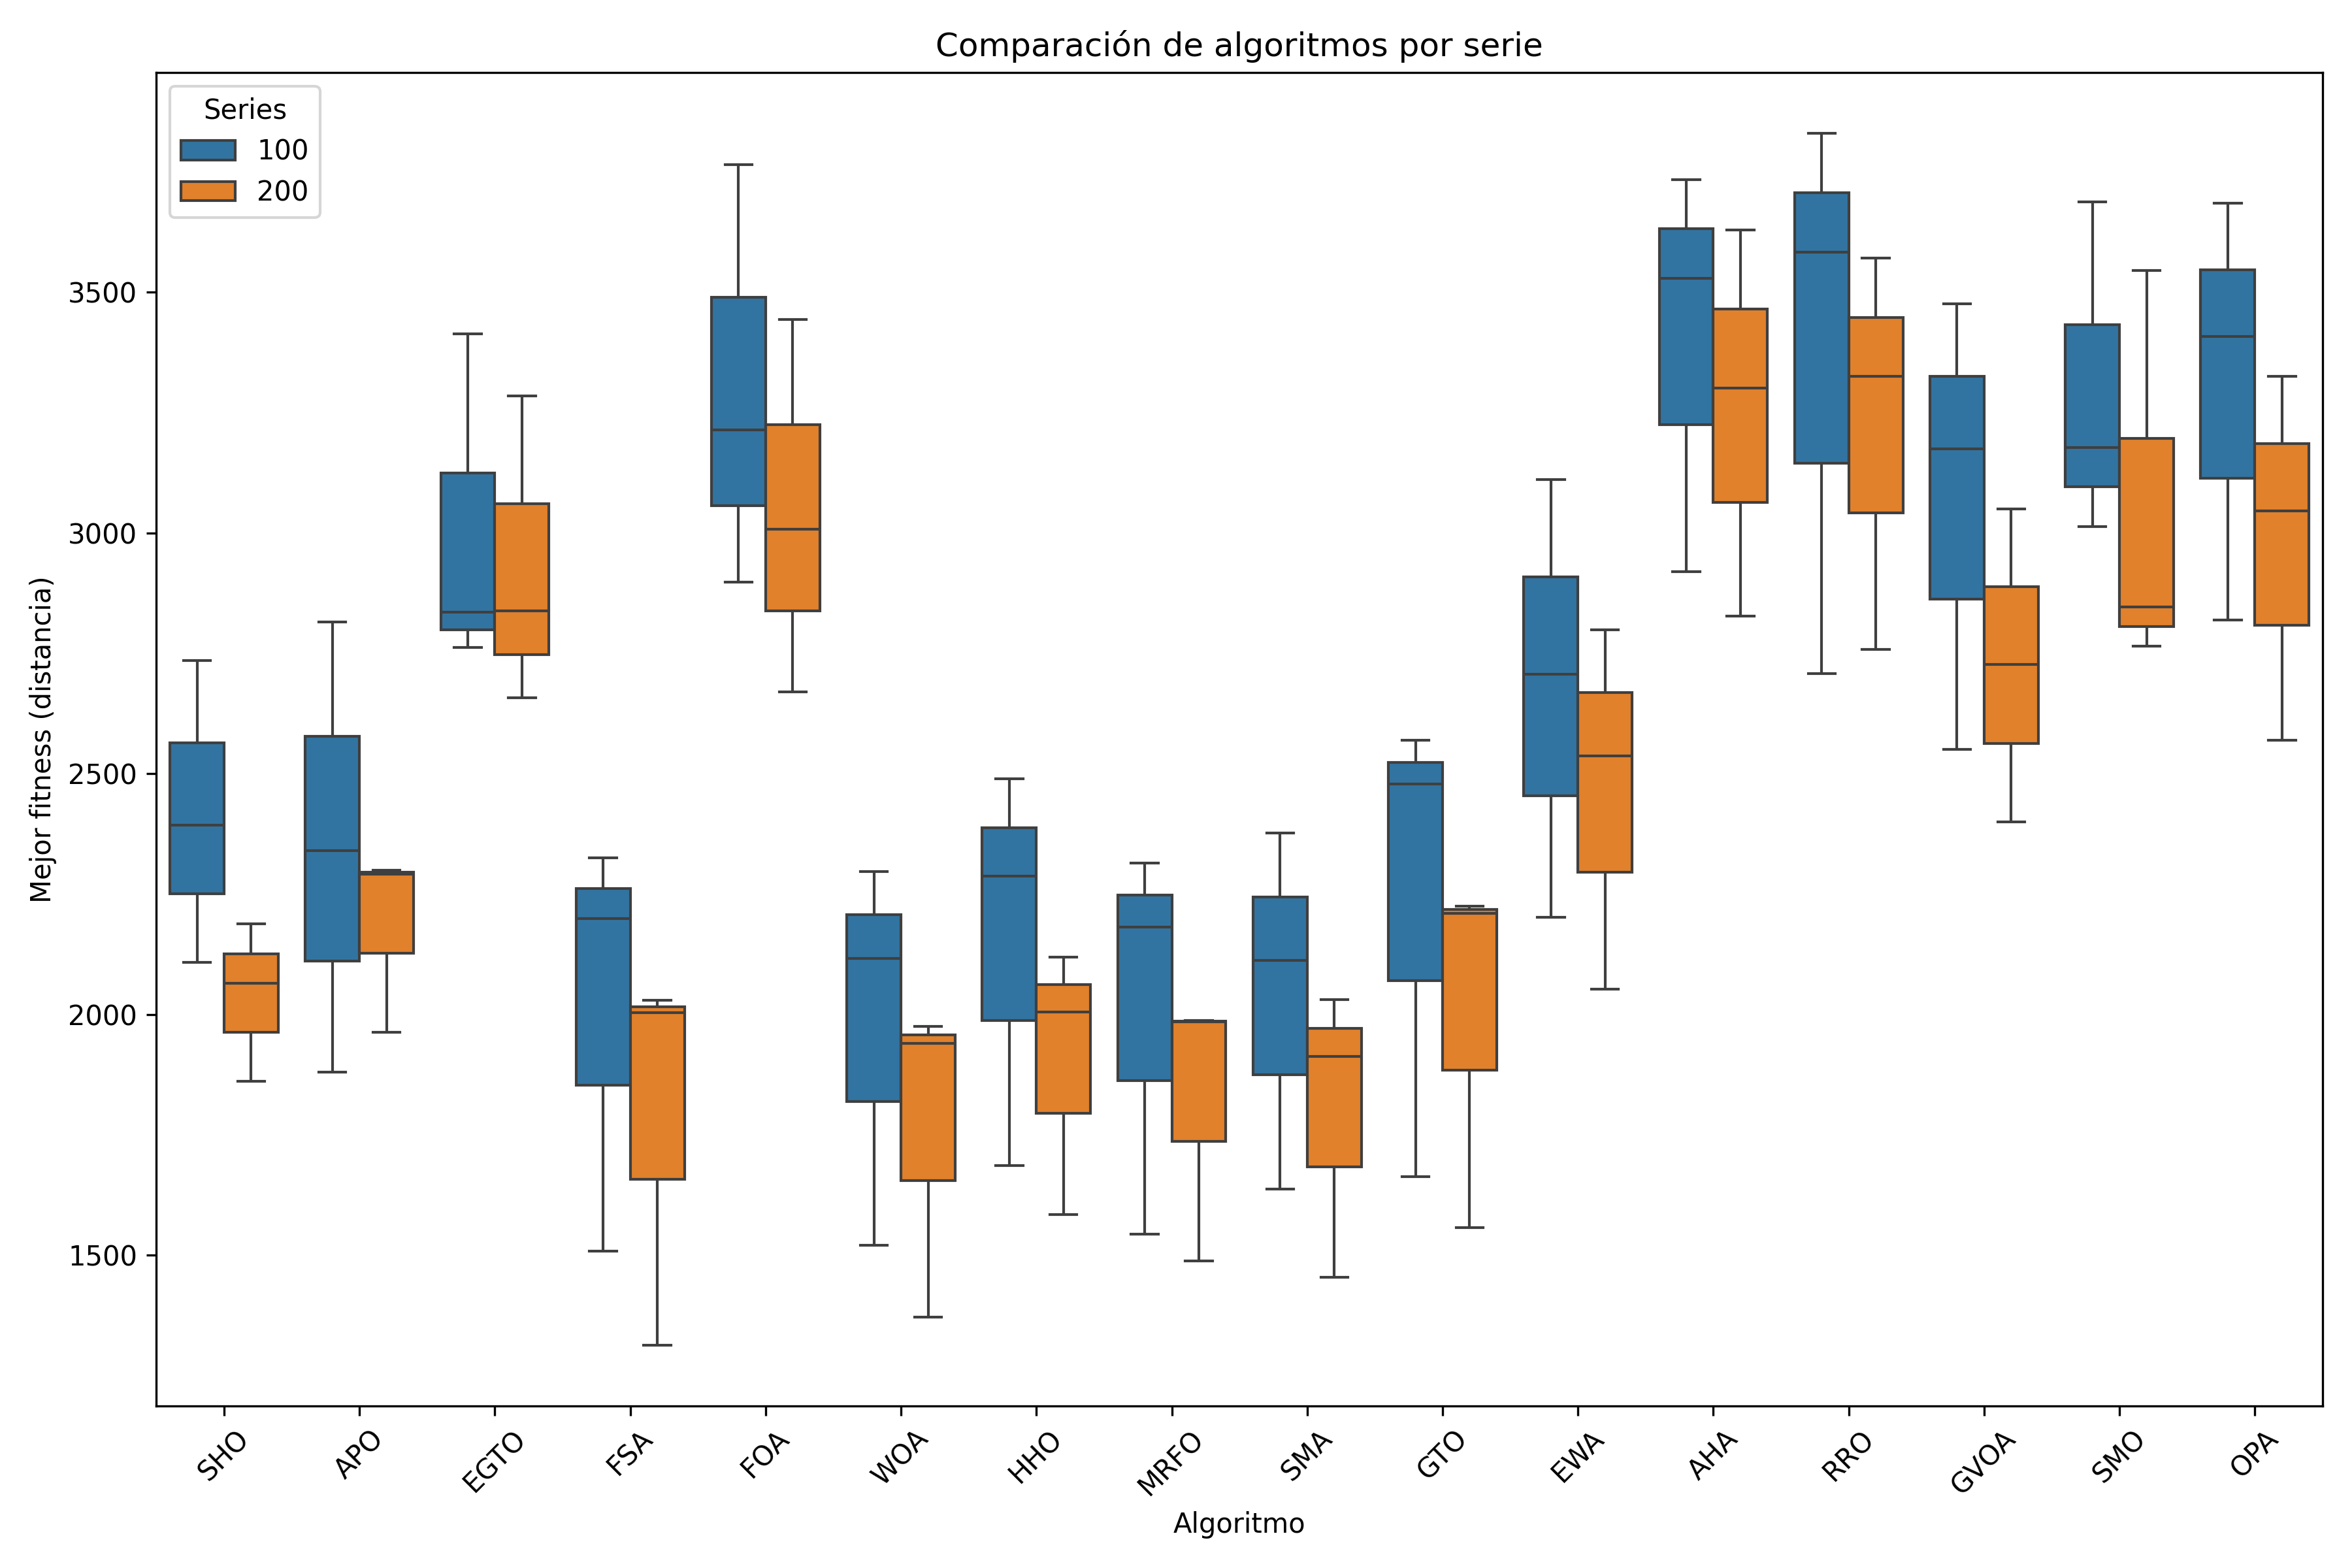
\includegraphics[width=\columnwidth]{benchmark_comparisons/solomon_final/algoritmos_por_serie.png}
  \caption{Comparación de fitness por tipo de instancia Solomon.}
  \label{fig:series}
\end{figure}

La Fig.~\ref{fig:series} revela otro patrón interesante: los algoritmos muestran comportamiento diferenciado entre las series 101 y 201. Algoritmos como WOA y FSA parecen adaptarse mejor a las restricciones temporales estrechas de las series 201.

\subsection{Interpretación Biológica del Rendimiento}

Resulta interesante que los algoritmos del grupo élite —WOA, FSA, MRFO y SMA— comparten características inspiradas en estrategias de búsqueda de alimento eficientes:

\begin{itemize}
\item WOA implementa la estrategia de "burbuja en red" de las ballenas jorobadas, un método de caza altamente cooperativo
\item MRFO combina tres estrategias de alimentación complementarias de las mantarrayas
\item SMA modela la adaptación dinámica del moho viscoso ante diferentes distribuciones de recursos
\item FSA simula comportamientos de filtración precisos y movimientos socialmente influenciados
\end{itemize}

Esto sugiere que las metáforas biológicas más efectivas para VRP podrían ser aquellas basadas en comportamientos de "foraging" (búsqueda de alimentos) con componentes de adaptación dinámica y cooperación, más que estrategias simples de depredación.

% Conclusiones
\section{Conclusiones y Trabajo Futuro}

Este estudio presenta una evaluación comparativa rigurosa de dieciséis algoritmos metaheurísticos bioinspirados aplicados al problema VRP. Las principales conclusiones son:

\begin{enumerate}
\item El análisis estadístico avanzado establece cuatro grupos de rendimiento estadísticamente diferenciados, con WOA, FSA, MRFO y SMA formando el grupo de élite sin diferencias significativas entre ellos.
\item SMA ofrece el mejor equilibrio calidad/coste, requiriendo aproximadamente la mitad del tiempo computacional que WOA con calidad de solución equivalente.
\item Los algoritmos muestran comportamiento diferenciado según el tipo de instancia, sugiriendo potencial para estrategias de selección adaptativa.
\item El análisis de tamaños de efecto A12 complementa la significancia estadística, cuantificando la magnitud práctica de las diferencias entre algoritmos.
\end{enumerate}

Como trabajo futuro, proponemos:

\begin{enumerate}
\item Evaluar el rendimiento en instancias de mayor tamaño (Homberger, 200-400 clientes) para analizar la escalabilidad de los algoritmos.
\item Implementar un análisis de sensibilidad para examinar el impacto de parámetros críticos (población, iteraciones) en la calidad de solución y tiempo de ejecución.
\item Desarrollar algoritmos híbridos que combinen las estrategias más efectivas identificadas en este estudio.
\item Extender el análisis a otros problemas de optimización combinatoria para evaluar la generalidad de nuestros hallazgos.
\end{enumerate}

\section{Apéndice de Reproducibilidad}

Para garantizar la reproducibilidad completa de este estudio, ponemos a disposición de la comunidad científica los siguientes recursos:

\begin{itemize}
\item Código fuente completo: \url{https://github.com/kaosb/BioAlgoCompare/releases/tag/v1.0.0}
\item Datos de benchmarking: \texttt{results/bio16\_solomon\_timed/massive\_benchmark\_summary.csv}
\item Comandos para reproducir el análisis:

\begin{verbatim}
# Ejecutar benchmarks masivos
python scripts/run_massive.py \
    --instances "C101,R101,RC101,C201,R201,RC201" \
    --algorithms "egto,foa,woa,hho,mrfo,sma" \
    --runs 1000 --iterations 100 --population 40 \
    --parallel

# Generar análisis estadístico
python scripts/analyze.py stats \
    --csv results/bio16_solomon_timed/massive_benchmark_summary.csv \
    --out benchmark_comparisons/solomon_final
\end{verbatim}
\end{itemize}

% Referencias
\selectlanguage{english}
\bibliographystyle{IEEEtran}
\bibliography{docs/references}

\begin{thebibliography}{1}

\bibitem{bioalgocompare_v1}
F. I.~González, ``BioAlgoCompare,'' 2025. [Online]. Available: \url{https://github.com/kaosb/BioAlgoCompare}, version = {v1.0.0}

\end{thebibliography}

\end{document}